\documentclass{article}

\usepackage{graphicx}
\usepackage{tikz}
\usepackage{tikzsymbols}
\usetikzlibrary{calc,patterns,shapes.geometric}
\pagestyle{empty}
\usepackage[margin=0pt]{geometry}
\geometry{papersize={14in,12in}}

\def\centerarc[#1](#2)(#3:#4:#5){\draw[#1] ($(#2)+({#5*cos(#3)},{#5*sin(#3)})$) arc (#3:#4:#5);}

\begin{document}
	\begin{figure}
		\centering
		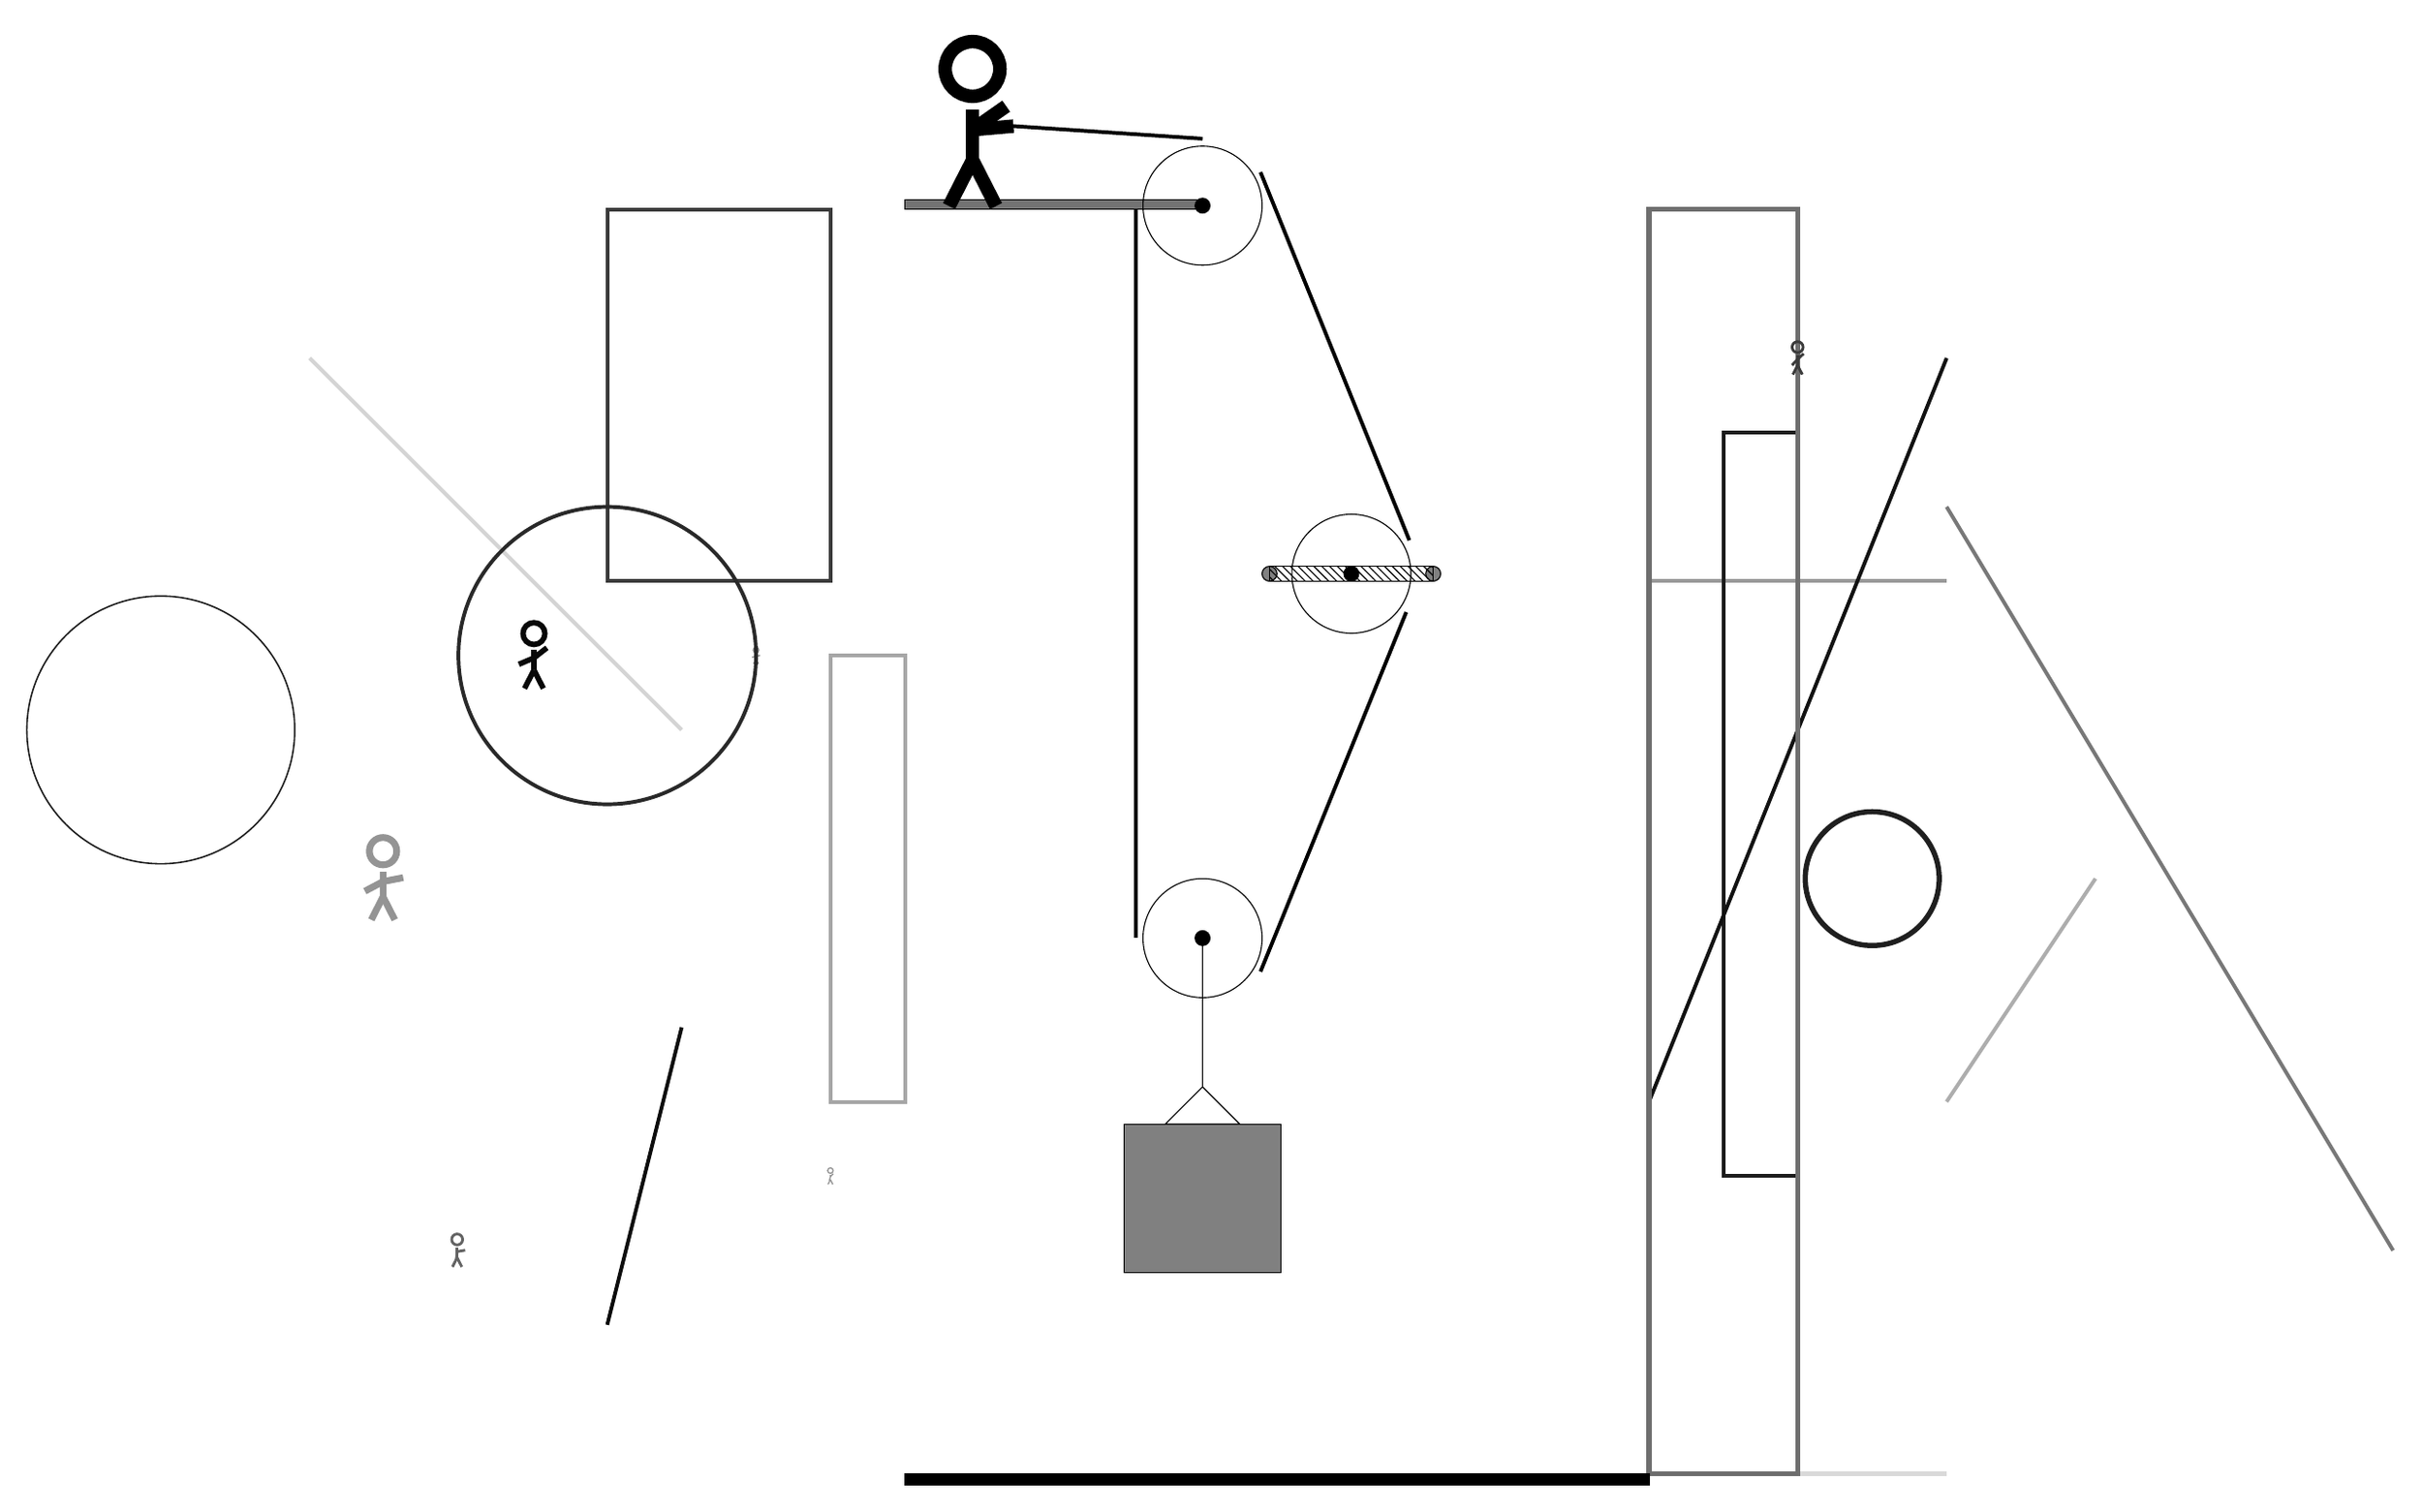
\begin{tikzpicture}
			%%%%% START %%%%%
			
			\draw[fill=black!55] (-2, 14) rectangle (2, 14.125);
			
			\draw (2, 4.2) circle (0.8);
			\draw[fill=black] (2, 4.2) circle (0.1);
			
			\draw (2, 14.05) circle (0.8);
			\draw[fill=black] (2, 14.05) circle (0.1);
			
			\draw[fill=white](4, 9.1) circle (0.8);
			\draw[fill=black] (4, 9.1) circle (0.1);
			\draw[fill=black!50] (2.9, 9.1) circle (0.1);
			\draw[fill=black!50] (5.1, 9.1) circle (0.1);
			\draw[pattern=north west lines, pattern color=black] (2.9, 9.2) rectangle (5.1, 9.0);
			
			\draw (2, 4.2) -- (2, 2.2) -- (1.5, 1.7) -- (2.5, 1.7) -- (2, 2.2);
			\draw[fill=black!50] (0.95, 1.7) rectangle (3.05, -0.3);
			
			\node[line width=0.2mm, color=black!97] at (-7, 8) {\Strichmaxerl[4][23][38]};
			
			\draw[line width=0.5mm, color=black!77] (-3, 14) rectangle (-6, 9);
			\node[line width=0.5mm, color=black!42] at (-9, 5) {\Strichmaxerl[5][28][11]};
			\node[line width=0.5mm, color=black!61] at (-8, 0) {\Strichmaxerl[2][84][10]};
			\draw [line width=0.2mm, color=black!89](-12, 7) circle (1.8);
			\draw[line width=0.5mm, color=black!95](-6, -1) -- (-5, 3);
			
			\draw[line width=0.7mm, color=black!18] (8, 0) rectangle (8, -1);
			\draw[line width=0.5mm, color=black!32](12, 2) -- (14, 5);
			\draw[line width=0.5mm, color=black!53](12, 10) -- (18, 0);
			
			\draw[line width=0.5mm, color=black!17](-5, 7) -- (-10, 12);
			\draw[line width=0.5mm, color=black!35] (-2, 2) rectangle (-3, 8);
			\node[line width=0.3mm, color=black!47] at (-4, 8) {\Strichmaxerl[1][16][10]};
			\draw[line width=0.5mm, color=black!40](8, 9) -- (12, 9);
			
			\draw[line width=0.5mm, color=black!89] (10, 1) rectangle (9, 11);
			\draw[line width=0.7mm, color=black!15] (10, -3) rectangle (12, -3);
			\draw[line width=0.5mm, color=black!93](12, 12) -- (8, 2);
			
			\draw[line width=0.7mm, color=black!57] (10, -3) rectangle (8, 14);
			\node[line width=0.2mm, color=black!77] at (10, 12) {\Strichmaxerl[2][47][43]};
			\node[line width=0.2mm, color=black!40] at (-3, 1) {\Strichmaxerl[1][77][45]};
			\draw [line width=0.5mm, color=black!84](-6, 8) circle (2.0);
			\draw [line width=0.7mm, color=black!88](11, 5) circle (0.9);
			
			
			\draw[line width=0.5mm] (1.1, 14) -- (1.1, 4.2);
			\centerarc[line width=0.5mm](2, 4.2)(180:330:0.9);
			\draw[line width=0.5mm](2.7794, 3.75) -- (4.7373, 8.5838);
			\centerarc[line width=0.5mm](4, 9.1)(390:325:0.9);
			\draw[line width=0.5mm](4.7794, 9.55) -- (2.7794, 14.5);
			\centerarc[line width=0.5mm](2, 14.05)(30:90:0.9);
			\draw[line width=0.5mm](2, 14.95) -- (-1, 15.15);
			
			\node at (-1, 15.15) {\Strichmaxerl[10][-175][35]};
			
			\draw[fill=black] (-2, -3) rectangle (8, -3.15);
			
			%%%%% END %%%%%
		\end{tikzpicture}
	\end{figure}	
\end{document}